% Created by tikzDevice version 0.12.6 on 2024-06-15 18:34:54
% !TEX encoding = UTF-8 Unicode
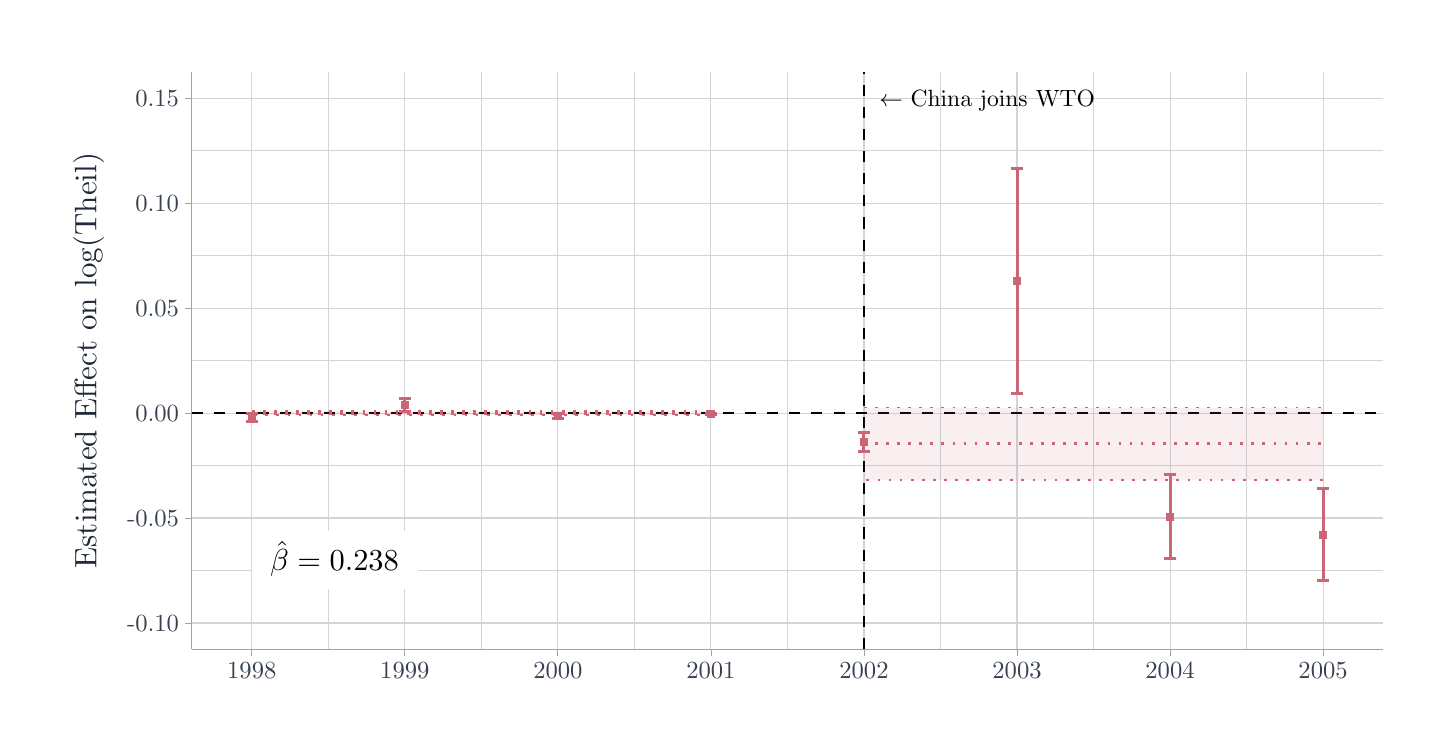
\begin{tikzpicture}[x=1pt,y=1pt]
\definecolor{fillColor}{RGB}{255,255,255}
\path[use as bounding box,fill=fillColor] (0,0) rectangle (505.89,252.94);
\begin{scope}
\path[clip] (  0.00,  0.00) rectangle (505.89,252.94);
\definecolor{drawColor}{RGB}{255,255,255}

\path[draw=drawColor,line width= 0.5pt,line join=round,line cap=round,fill=fillColor] (  0.00,  0.00) rectangle (505.89,252.94);
\end{scope}
\begin{scope}
\path[clip] ( 59.20, 28.35) rectangle (489.89,236.94);
\definecolor{drawColor}{RGB}{255,255,255}
\definecolor{fillColor}{RGB}{255,255,255}

\path[draw=drawColor,line width= 0.5pt,line join=round,line cap=round,fill=fillColor] ( 59.20, 28.35) rectangle (489.89,236.94);
\definecolor{drawColor}{RGB}{209,213,219}

\path[draw=drawColor,line width= 0.4pt,line join=round] ( 59.20, 56.79) --
	(489.89, 56.79);

\path[draw=drawColor,line width= 0.4pt,line join=round] ( 59.20, 94.72) --
	(489.89, 94.72);

\path[draw=drawColor,line width= 0.4pt,line join=round] ( 59.20,132.65) --
	(489.89,132.65);

\path[draw=drawColor,line width= 0.4pt,line join=round] ( 59.20,170.57) --
	(489.89,170.57);

\path[draw=drawColor,line width= 0.4pt,line join=round] ( 59.20,208.50) --
	(489.89,208.50);

\path[draw=drawColor,line width= 0.4pt,line join=round] (108.64, 28.35) --
	(108.64,236.94);

\path[draw=drawColor,line width= 0.4pt,line join=round] (163.94, 28.35) --
	(163.94,236.94);

\path[draw=drawColor,line width= 0.4pt,line join=round] (219.24, 28.35) --
	(219.24,236.94);

\path[draw=drawColor,line width= 0.4pt,line join=round] (274.54, 28.35) --
	(274.54,236.94);

\path[draw=drawColor,line width= 0.4pt,line join=round] (329.85, 28.35) --
	(329.85,236.94);

\path[draw=drawColor,line width= 0.4pt,line join=round] (385.15, 28.35) --
	(385.15,236.94);

\path[draw=drawColor,line width= 0.4pt,line join=round] (440.45, 28.35) --
	(440.45,236.94);

\path[draw=drawColor,line width= 0.4pt,line join=round] ( 59.20, 37.83) --
	(489.89, 37.83);

\path[draw=drawColor,line width= 0.4pt,line join=round] ( 59.20, 75.76) --
	(489.89, 75.76);

\path[draw=drawColor,line width= 0.4pt,line join=round] ( 59.20,113.68) --
	(489.89,113.68);

\path[draw=drawColor,line width= 0.4pt,line join=round] ( 59.20,151.61) --
	(489.89,151.61);

\path[draw=drawColor,line width= 0.4pt,line join=round] ( 59.20,189.54) --
	(489.89,189.54);

\path[draw=drawColor,line width= 0.4pt,line join=round] ( 59.20,227.46) --
	(489.89,227.46);

\path[draw=drawColor,line width= 0.4pt,line join=round] ( 80.99, 28.35) --
	( 80.99,236.94);

\path[draw=drawColor,line width= 0.4pt,line join=round] (136.29, 28.35) --
	(136.29,236.94);

\path[draw=drawColor,line width= 0.4pt,line join=round] (191.59, 28.35) --
	(191.59,236.94);

\path[draw=drawColor,line width= 0.4pt,line join=round] (246.89, 28.35) --
	(246.89,236.94);

\path[draw=drawColor,line width= 0.4pt,line join=round] (302.19, 28.35) --
	(302.19,236.94);

\path[draw=drawColor,line width= 0.4pt,line join=round] (357.50, 28.35) --
	(357.50,236.94);

\path[draw=drawColor,line width= 0.4pt,line join=round] (412.80, 28.35) --
	(412.80,236.94);

\path[draw=drawColor,line width= 0.4pt,line join=round] (468.10, 28.35) --
	(468.10,236.94);
\definecolor{drawColor}{RGB}{0,0,0}

\path[draw=drawColor,line width= 0.6pt,dash pattern=on 4pt off 4pt ,line join=round] ( 59.20,113.68) -- (489.89,113.68);

\path[draw=drawColor,line width= 0.6pt,dash pattern=on 4pt off 4pt ,line join=round] (302.19, 28.35) -- (302.19,236.94);

\node[text=drawColor,anchor=base west,inner sep=0pt, outer sep=0pt, scale=  0.85] at (307.72,224.52) {$\leftarrow$ China joins WTO};

\path[fill=fillColor] ( 80.99, 50.14) --
	(140.98, 50.14) --
	(140.98, 50.14) --
	(140.98, 50.14) --
	(140.98, 50.14) --
	(140.98, 50.14) --
	(140.98, 50.14) --
	(140.98, 50.14) --
	(140.98, 50.14) --
	(140.98, 50.14) --
	(140.98, 50.14) --
	(140.98, 50.14) --
	(140.98, 50.14) --
	(140.98, 50.14) --
	(140.98, 71.04) --
	(140.98, 71.04) --
	(140.98, 71.04) --
	(140.98, 71.04) --
	(140.98, 71.04) --
	(140.98, 71.04) --
	(140.98, 71.04) --
	(140.98, 71.04) --
	(140.98, 71.04) --
	(140.98, 71.04) --
	(140.98, 71.04) --
	(140.98, 71.04) --
	( 80.99, 71.04) --
	( 80.99, 71.04) --
	( 80.99, 71.04) --
	( 80.99, 71.04) --
	( 80.99, 71.04) --
	( 80.99, 71.04) --
	( 80.99, 71.04) --
	( 80.99, 71.04) --
	( 80.99, 71.04) --
	( 80.99, 71.04) --
	( 80.99, 71.04) --
	( 80.99, 71.04) --
	( 80.99, 71.04) --
	( 80.99, 50.14) --
	( 80.99, 50.14) --
	( 80.99, 50.14) --
	( 80.99, 50.14) --
	( 80.99, 50.14) --
	( 80.99, 50.14) --
	( 80.99, 50.14) --
	( 80.99, 50.14) --
	( 80.99, 50.14) --
	( 80.99, 50.14) --
	( 80.99, 50.14) --
	( 80.99, 50.14) --
	cycle;
\end{scope}
\begin{scope}
\path[clip] ( 59.20, 28.35) rectangle (489.89,236.94);
\definecolor{drawColor}{RGB}{0,0,0}

\node[text=drawColor,anchor=base west,inner sep=0pt, outer sep=0pt, scale=  1.10] at ( 87.63, 56.79) {$\hat{\beta} = 0.238$};
\end{scope}
\begin{scope}
\path[clip] ( 59.20, 28.35) rectangle (489.89,236.94);
\definecolor{drawColor}{RGB}{204,102,119}

\path[draw=drawColor,line width= 1.1pt,line join=round] ( 78.77,113.41) --
	( 83.20,113.41);

\path[draw=drawColor,line width= 1.1pt,line join=round] ( 80.99,113.41) --
	( 80.99,110.64);

\path[draw=drawColor,line width= 1.1pt,line join=round] ( 78.77,110.64) --
	( 83.20,110.64);

\path[draw=drawColor,line width= 1.1pt,line join=round] (134.08,119.08) --
	(138.50,119.08);

\path[draw=drawColor,line width= 1.1pt,line join=round] (136.29,119.08) --
	(136.29,114.28);

\path[draw=drawColor,line width= 1.1pt,line join=round] (134.08,114.28) --
	(138.50,114.28);

\path[draw=drawColor,line width= 1.1pt,line join=round] (189.38,113.51) --
	(193.80,113.51);

\path[draw=drawColor,line width= 1.1pt,line join=round] (191.59,113.51) --
	(191.59,111.64);

\path[draw=drawColor,line width= 1.1pt,line join=round] (189.38,111.64) --
	(193.80,111.64);

\path[draw=drawColor,line width= 1.1pt,line join=round] (244.68,113.65) --
	(249.10,113.65);

\path[draw=drawColor,line width= 1.1pt,line join=round] (246.89,113.65) --
	(246.89,113.27);

\path[draw=drawColor,line width= 1.1pt,line join=round] (244.68,113.27) --
	(249.10,113.27);

\path[draw=drawColor,line width= 1.1pt,line join=round] (299.98,106.67) --
	(304.41,106.67);

\path[draw=drawColor,line width= 1.1pt,line join=round] (302.19,106.67) --
	(302.19, 99.64);

\path[draw=drawColor,line width= 1.1pt,line join=round] (299.98, 99.64) --
	(304.41, 99.64);

\path[draw=drawColor,line width= 1.1pt,line join=round] (355.28,201.98) --
	(359.71,201.98);

\path[draw=drawColor,line width= 1.1pt,line join=round] (357.50,201.98) --
	(357.50,120.66);

\path[draw=drawColor,line width= 1.1pt,line join=round] (355.28,120.66) --
	(359.71,120.66);

\path[draw=drawColor,line width= 1.1pt,line join=round] (410.59, 91.43) --
	(415.01, 91.43);

\path[draw=drawColor,line width= 1.1pt,line join=round] (412.80, 91.43) --
	(412.80, 61.05);

\path[draw=drawColor,line width= 1.1pt,line join=round] (410.59, 61.05) --
	(415.01, 61.05);

\path[draw=drawColor,line width= 1.1pt,line join=round] (465.89, 86.27) --
	(470.31, 86.27);

\path[draw=drawColor,line width= 1.1pt,line join=round] (468.10, 86.27) --
	(468.10, 53.02);

\path[draw=drawColor,line width= 1.1pt,line join=round] (465.89, 53.02) --
	(470.31, 53.02);
\definecolor{fillColor}{RGB}{204,102,119}

\path[fill=fillColor] ( 79.56,110.60) --
	( 82.41,110.60) --
	( 82.41,113.45) --
	( 79.56,113.45) --
	cycle;

\path[fill=fillColor] (134.86,115.25) --
	(137.71,115.25) --
	(137.71,118.11) --
	(134.86,118.11) --
	cycle;

\path[fill=fillColor] (190.16,111.14) --
	(193.02,111.14) --
	(193.02,114.00) --
	(190.16,114.00) --
	cycle;

\path[fill=fillColor] (245.47,112.03) --
	(248.32,112.03) --
	(248.32,114.89) --
	(245.47,114.89) --
	cycle;

\path[fill=fillColor] (300.77,101.73) --
	(303.62,101.73) --
	(303.62,104.58) --
	(300.77,104.58) --
	cycle;

\path[fill=fillColor] (356.07,159.89) --
	(358.92,159.89) --
	(358.92,162.75) --
	(356.07,162.75) --
	cycle;

\path[fill=fillColor] (411.37, 74.81) --
	(414.23, 74.81) --
	(414.23, 77.67) --
	(411.37, 77.67) --
	cycle;

\path[fill=fillColor] (466.67, 68.22) --
	(469.53, 68.22) --
	(469.53, 71.07) --
	(466.67, 71.07) --
	cycle;
\definecolor{fillColor}{RGB}{204,102,119}

\path[fill=fillColor,fill opacity=0.10] (302.19,115.64) --
	(468.10,115.64) --
	(468.10, 89.54) --
	(302.19, 89.54) --
	cycle;

\path[draw=drawColor,line width= 0.6pt,dash pattern=on 1pt off 3pt ,line join=round] (302.19,115.64) --
	(468.10,115.64);

\path[draw=drawColor,line width= 0.6pt,dash pattern=on 1pt off 3pt ,line join=round] (468.10, 89.54) --
	(302.19, 89.54);

\path[fill=fillColor,fill opacity=0.10] ( 80.99,114.48) --
	(246.89,114.48) --
	(246.89,112.89) --
	( 80.99,112.89) --
	cycle;

\path[draw=drawColor,line width= 0.6pt,dash pattern=on 1pt off 3pt ,line join=round] ( 80.99,114.48) --
	(246.89,114.48);

\path[draw=drawColor,line width= 0.6pt,dash pattern=on 1pt off 3pt ,line join=round] (246.89,112.89) --
	( 80.99,112.89);

\path[draw=drawColor,line width= 1.1pt,dash pattern=on 1pt off 3pt ,line join=round] (302.19,102.59) --
	(468.10,102.59);

\path[draw=drawColor,line width= 1.1pt,dash pattern=on 1pt off 3pt ,line join=round] ( 80.99,113.68) --
	(246.89,113.68);
\end{scope}
\begin{scope}
\path[clip] (  0.00,  0.00) rectangle (505.89,252.94);
\definecolor{drawColor}{RGB}{156,163,175}

\path[draw=drawColor,line width= 0.3pt,line join=round] ( 59.20, 28.35) --
	( 59.20,236.94);
\end{scope}
\begin{scope}
\path[clip] (  0.00,  0.00) rectangle (505.89,252.94);
\definecolor{drawColor}{RGB}{55,65,81}

\node[text=drawColor,anchor=base east,inner sep=0pt, outer sep=0pt, scale=  0.89] at ( 54.70, 34.77) {-0.10};

\node[text=drawColor,anchor=base east,inner sep=0pt, outer sep=0pt, scale=  0.89] at ( 54.70, 72.70) {-0.05};

\node[text=drawColor,anchor=base east,inner sep=0pt, outer sep=0pt, scale=  0.89] at ( 54.70,110.62) {0.00};

\node[text=drawColor,anchor=base east,inner sep=0pt, outer sep=0pt, scale=  0.89] at ( 54.70,148.55) {0.05};

\node[text=drawColor,anchor=base east,inner sep=0pt, outer sep=0pt, scale=  0.89] at ( 54.70,186.48) {0.10};

\node[text=drawColor,anchor=base east,inner sep=0pt, outer sep=0pt, scale=  0.89] at ( 54.70,224.40) {0.15};
\end{scope}
\begin{scope}
\path[clip] (  0.00,  0.00) rectangle (505.89,252.94);
\definecolor{drawColor}{RGB}{156,163,175}

\path[draw=drawColor,line width= 0.3pt,line join=round] ( 56.70, 37.83) --
	( 59.20, 37.83);

\path[draw=drawColor,line width= 0.3pt,line join=round] ( 56.70, 75.76) --
	( 59.20, 75.76);

\path[draw=drawColor,line width= 0.3pt,line join=round] ( 56.70,113.68) --
	( 59.20,113.68);

\path[draw=drawColor,line width= 0.3pt,line join=round] ( 56.70,151.61) --
	( 59.20,151.61);

\path[draw=drawColor,line width= 0.3pt,line join=round] ( 56.70,189.54) --
	( 59.20,189.54);

\path[draw=drawColor,line width= 0.3pt,line join=round] ( 56.70,227.46) --
	( 59.20,227.46);
\end{scope}
\begin{scope}
\path[clip] (  0.00,  0.00) rectangle (505.89,252.94);
\definecolor{drawColor}{RGB}{156,163,175}

\path[draw=drawColor,line width= 0.3pt,line join=round] ( 59.20, 28.35) --
	(489.89, 28.35);
\end{scope}
\begin{scope}
\path[clip] (  0.00,  0.00) rectangle (505.89,252.94);
\definecolor{drawColor}{RGB}{156,163,175}

\path[draw=drawColor,line width= 0.3pt,line join=round] ( 80.99, 25.85) --
	( 80.99, 28.35);

\path[draw=drawColor,line width= 0.3pt,line join=round] (136.29, 25.85) --
	(136.29, 28.35);

\path[draw=drawColor,line width= 0.3pt,line join=round] (191.59, 25.85) --
	(191.59, 28.35);

\path[draw=drawColor,line width= 0.3pt,line join=round] (246.89, 25.85) --
	(246.89, 28.35);

\path[draw=drawColor,line width= 0.3pt,line join=round] (302.19, 25.85) --
	(302.19, 28.35);

\path[draw=drawColor,line width= 0.3pt,line join=round] (357.50, 25.85) --
	(357.50, 28.35);

\path[draw=drawColor,line width= 0.3pt,line join=round] (412.80, 25.85) --
	(412.80, 28.35);

\path[draw=drawColor,line width= 0.3pt,line join=round] (468.10, 25.85) --
	(468.10, 28.35);
\end{scope}
\begin{scope}
\path[clip] (  0.00,  0.00) rectangle (505.89,252.94);
\definecolor{drawColor}{RGB}{55,65,81}

\node[text=drawColor,anchor=base,inner sep=0pt, outer sep=0pt, scale=  0.89] at ( 80.99, 17.73) {1998};

\node[text=drawColor,anchor=base,inner sep=0pt, outer sep=0pt, scale=  0.89] at (136.29, 17.73) {1999};

\node[text=drawColor,anchor=base,inner sep=0pt, outer sep=0pt, scale=  0.89] at (191.59, 17.73) {2000};

\node[text=drawColor,anchor=base,inner sep=0pt, outer sep=0pt, scale=  0.89] at (246.89, 17.73) {2001};

\node[text=drawColor,anchor=base,inner sep=0pt, outer sep=0pt, scale=  0.89] at (302.19, 17.73) {2002};

\node[text=drawColor,anchor=base,inner sep=0pt, outer sep=0pt, scale=  0.89] at (357.50, 17.73) {2003};

\node[text=drawColor,anchor=base,inner sep=0pt, outer sep=0pt, scale=  0.89] at (412.80, 17.73) {2004};

\node[text=drawColor,anchor=base,inner sep=0pt, outer sep=0pt, scale=  0.89] at (468.10, 17.73) {2005};
\end{scope}
\begin{scope}
\path[clip] (  0.00,  0.00) rectangle (505.89,252.94);
\definecolor{drawColor}{RGB}{31,41,55}

\node[text=drawColor,rotate= 90.00,anchor=base,inner sep=0pt, outer sep=0pt, scale=  1.12] at ( 24.84,132.65) {Estimated Effect on $\log($Theil$)$};
\end{scope}
\end{tikzpicture}
